\fancychapter{Implementation}
\label{chap:imp}

This chapter presents the implementation of the \acs{mppt} charger prototype. The charger is based on a synchronous boost converter controlled by an STM32 \acs{mcu}, with dedicated sensing, protection, communication and configuration features.

The chapter first describes the \acs{dc}--\acs{dc} converter, including its operating principles and the dimensioning of the main power components. The processing unit and its configuration are then presented, followed by the voltage, current, temperature and irradiance sensing circuits. Finally, the firmware architecture is described, covering the charging state machine, communication interfaces and the graphical user interface used to configure the device.

\section{DC-DC converter}

Since the solar panels voltage of \ac{sg01} are always lower than the battery voltage, a step-up converter is required. This section presents its operating principles and the dimensioning of the main components.

\subsection{Operation principles}
The DC-DC converter chosen for this project was a boost converter. This topology uses one switching device, one inductor, one output capacitor, and a diode, Figure \ref{fig:boost}. The switching device is used to control the output voltage by switching on and off at a specified frequency (fsw) and duty cycle (D). The inductor is used to store energy when the switch is on (stage 1) and release it when the switch is off (stage 2), while the output capacitor is used to smooth the output voltage.

\begin{figure}[!ht]
    \centering
    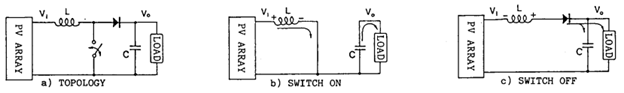
\includegraphics[width=0.9\textwidth]{Images/Implementation/Boost.png}
    \caption{Classic boost converter topology and stages \cite{Comparison_PV_Converter_Technologies_1989}.}
    \label{fig:boost}
\end{figure}

Analyzing the boost converter separately in its two stages, it is possible to define the voltage drop across the inductor (VL), as a function of the input voltage (Vin) and output voltage (Vout) as follows:

\begin{equation}
    V_L = \begin{cases}
    V_{in} & \text{if } t \in [0, D \cdot T] \\
    V_{in} - V_{out} & \text{if } t \in [D \cdot T, T]
  \end{cases}
  \label{eq:vl}
\end{equation}

With equation \ref{eq:vl} and the fact that at the stationary state the average voltage across the inductor is zero, it is possible to define the output voltage as a function of the input voltage and duty cycle as follows:

\begin{equation}
    V_{Lavg} = \frac{1}{T} (\int_{0}^{DT} V_{in} dt + \int_{DT}^{T} (V_{in} - V_{out}) dt) = 0 \Rightarrow V_{out} = \frac{V_{in}}{1-D}
    \label{eq:duty}
\end{equation}

Equation \ref{eq:duty} is one of the most important equations in boost converter design, as it defines the relationship between the input voltage, output voltage and duty cycle. As the duty cycle increases, the output voltage also increases, which is the main principle behind boost converters. For our use case, it is also important to analyze the relationship between the input and output current. Considering no power losses, it is possible to define the input current as follows:
\begin{equation}
    P_{in} = P_{out} \Leftrightarrow V_{in} \cdot I_{in} = V_{out} \cdot I_{out} \Leftrightarrow I_{in} = \frac{V_{out}}{V_{in}} \cdot I_{out} \Leftrightarrow I_{in} = \frac{I_{out}}{1-D}
\end{equation}

However, these equations are only valid for ideal components since they do not take into account the parasitic elements of the components, such as the inductor resistance, the drain-source resistance, and the voltage drop across the diode (there are other parasitic components that also affect performance). In a real boost converter, these parasitic elements will cause a voltage drop and therefore reduce the output voltage. 

The influence of the transistor internal resistance ($R_{DS_{(on)}}$), the inductor resistance ($R_L$) and the diode voltage drop ($V_d$) can be briefly evaluated by modifying Equation~\ref{eq:vl} as follows:

\begin{equation}
    V_L = \begin{cases}
    V_{in} - R_{DS_{(on)}} \cdot I_{DS} & \text{if } t \in [0, D \cdot T] \\
    V_{in} - V_{out} - V_d & \text{if } t \in [D \cdot T, T]
  \end{cases}
  \label{eq:vl2}
\end{equation}

In this case, at the stationary state, the average voltage across the inductor is $R_L \cdot I_L$ and therefore the output voltage can be defined as:

\begin{equation}
    V_{Lavg} = \frac{1}{T} (\int_{0}^{DT} (V_{in} - R_{DS_{(on)}} \cdot I_{DS}) dt + \int_{DT}^{T} (V_{in} - V_{out} - V_d) dt) \Leftrightarrow 
\end{equation}

\begin{equation}
    \Leftrightarrow R_L \cdot I_L = \frac{1}{T} [T \cdot D \cdot  (V_{in} - R_{DS_{(on)}} \cdot I_{DS}) + T \cdot (1-D)\cdot(V_{in} - V_{out} -V_d)] \Leftrightarrow 
    \label{eq:vout3}
\end{equation}

\begin{equation}
    \Leftrightarrow  V_{out} = \frac{V_{in} - D \cdot R_{DS_{(on)}} \cdot I_{DS} - R_L \cdot I_L}{1-D}-V_d
    \label{eq:vout2}
\end{equation}

Equation \ref{eq:vout2} shows the 3 causes of losses in a boost converter. The most significant is usually the voltage drop across the diode (typically 0.3~V to 0.7~V), which reduces the efficiency through a conduction loss of $V_d \cdot I_{out}$. This can be largely avoided by using a synchronous boost converter (Figure~\ref{fig:sync_boost}), which replaces the diode with a transistor. In this case, the voltage drop is only $R_{DS,on} \cdot I$, which is usually below 0.1~V.

As for the transistor and inductor internal resistance, it cannot be removed entirely, so it must be taken into account when designing the boost converter. Therefore, it is important to select components with low internal resistance to minimize losses and increase converter efficiency.

\begin{figure}[!ht]
    \centering
    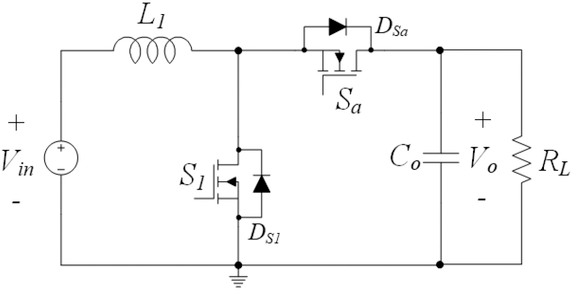
\includegraphics[width=0.5\textwidth]{Images/Implementation/Conventional-synchronous-boost-converter.png}
    \caption{Synchronous boost converter topology \cite{lee_high-efficiency_2019}.}
    \label{fig:sync_boost}
\end{figure}

\subsection{Dimensioning}
Let us first define the design goals of the synchronous boost converter. The converter must step up the voltage from the solar panels, which may consist of up to 40 cells (Maxeon Gen 3 from SunPower) connected in series, a minimum of 20 cells in series, and is optimized for 35 cells (Table~\ref{tab:pv_conditions}). 
The converter must charge a lithium-ion battery with a nominal voltage of 43.2~V. 
The switching frequency was defined as 100~kHz. This relatively high frequency allows the use of smaller inductors and capacitors, while still avoiding excessive switching losses.

Table~\ref{tab:converter_constraints} and \ref{tab:pv_conditions} summarizes the system requirements.



\begin{table}[!ht]
    \centering
    \caption{\acs{pv} panel parameters at \acs{mppt}.}
    \label{tab:pv_conditions}
    
    \begin{tabular}{lccccc}
        \hline
        Configuration & $V_{mppt}$ (V) & $I_{mppt}$ (A) & $P_{mppt}$ (W) & $V_{oc}$ (V) & $I_{sc}$ (A) \\
        \hline
        40 cells & 24.68 & 6.05 & 139.6 & 29 & 6.374 \\
        35 cells & 21.875 & 6.05 & 122.15 & 25.375 & 6.374 \\
        20 cells & 12.34 & 6.05 & 69.8 & 14.5 & 6.374 \\
        \hline
    \end{tabular}
\end{table}


\begin{table}[!ht]
    \centering
    \caption{Converter design constraints.}
    \label{tab:converter_constraints}
    
    \begin{tabular}{lc}
        \hline
        Parameter & Value \\
        \hline
        Battery voltage (nominal) & 43.2~V \\
        Battery voltage (max) & 50.4~V \\
        Battery voltage (min) & 30~V \\
        $\Delta V_o$ & 0.1~V \\
        $\Delta V_i$ & 0.5~V \\
        Efficiency & $> 90\%$ \\
        \hline
    \end{tabular}
\end{table}

Since the load is a battery, the output ripple voltage must be limited to avoid aging and heating. Also, the output voltage ripple must be low to avoid unexpected behavior in the electronic components connected to the battery. As for the input (the solar panel), the voltage ripple must be low for easier measurement and precise control. Therefore, the values presented in Table~\ref{tab:converter_constraints} were selected. 

\subsubsection{Inductor}
The inductor is one of the most important components in the boost converter since it is responsible for storing energy and releasing it to the load. 

The choice of inductor strongly influences converter performance. High inductance will generate low current ripple, however it generates losses due to its internal resistance. On the other hand, a smaller inductance will generate high current ripples, high stress in components, and high magnetic interference. These current ripples can cause the system to operate in \ac{dcm}. In \ac{dcm}, the inductor current reaches zero during the switching period, which means that the energy stored in the inductor is not enough to supply the load during the off time. This can cause high current and voltage ripples, which can damage the components and reduce the efficiency of the converter. Therefore, it is important to ensure that the inductance value is high enough to operate in \ac{ccm}.


The equation that describes the inductor is defined as:
\begin{equation}
    V_L = L \cdot \frac{di_L}{dt} = L \cdot \frac{\Delta I_l}{\Delta t} \Leftrightarrow L = \frac{V_L \Delta t}{\Delta I_L}
    \label{eq:inductor1}
\end{equation}

In the first stage (transistor in conduction mode), the voltage in the inductor is equal to the input voltage and it occurs for $D \cdot T$~s. Therefore, the inductor ripple current can be defined as follows:

\begin{equation}
    \Delta I_L = \frac{V_{in} \cdot D \cdot T}{L}
\end{equation}

The current ripple can be described using the ripple factor and the average inductor current as follows.
\begin{equation}
    r = \frac{\Delta I_L}{I_{L,avg}}
    \label{eq:riple factor}
\end{equation}

\begin{equation}
    I_{L,avg} = \frac{I_o}{1-D}
    \label{eq:ilavg}
\end{equation}

Using Equation~\ref{eq:ilavg}, \ref{eq:riple factor}, \ref{eq:inductor1} and \ref{eq:duty}, the following equation is achieved:

\begin{equation}
    L = \frac{V_L \Delta t}{\Delta I_L} = \frac{V_{in}DT}{\frac{I_or}{1-D}} = \frac{V_{in} (1-D)DT}{I_o \cdot r} = \frac{V_{out}(1-D)^2DT}{I_o \cdot r}
    \label{eq:L}
\end{equation}

The value of D that maximizes Equation~\ref{eq:L} is 1/3, which results in the critical inductance formula:

\begin{equation}
    MAX[(1-D)^2\cdot D]= (1-1/3)^2 \cdot 1/3= \frac{4}{27}
\end{equation}
\begin{equation}
    L_{critical} = \frac{4}{27} \cdot \frac{V_o}{I_o \cdot r \cdot f}
\end{equation}

Using the maximum battery voltage (50.4~V) and the maximum current ($I_{bat}+Margin=10~A$), and a ripple factor of 2, which is equivalent  to the \ac{ccm} limit, the following result is achieved:

\begin{equation}
    L_{critical} = \frac{4}{27} \cdot \frac{50.4}{10 \cdot 2 \cdot 100 \times 10^{3}} = 3.73~\mu\mathrm{H}
\end{equation}

This is a reference value, if used, it would highly stress the components, generating heat, magnetic interference and high current ripples. Therefore, the calculation was repeated, this time with a ripple factor of 0.4, which is more reasonable. 

\begin{equation}
    L_{critical} = \frac{4}{27} \cdot \frac{50.4}{10 \cdot 0.4 \cdot 100 \times 10^{3}} = 18.66~\mu\mathrm{H}
\end{equation}

As it is explained in the simulation section (Section~\ref{chap:sims}), a higher value will be beneficial to reduce current ripple and noise. For that reason, the final inductor value was defined as $68~\mu\mathrm{H}$, which results in a ripple factor of 0.11.

To select the appropriate inductor, the rated current and the saturation current must be taken into account. The rated current is the maximum current that the inductor can handle without overheating. In this case, the rated current must be higher than the maximum short-circuit current of the biggest solar panel configuration (40 cells in series), which is 6.374~A. Some margin must be added to this value, so the rated current must be higher than 10~A.

The saturation current is the maximum current that the inductor can handle without saturating. When the inductor saturates, the inductance drops significantly, which can cause high current ripples and damage the components. Considering the Open circuit voltage of a 40 cells solar panel (worst case), the inductor ripple current is 4.26~A at 100\% duty cycle. Therefore, the saturation current must be:

\begin{equation}
    I_{sat} > I_{in} + \frac{\Delta I_L}{2} = 6.374 + \frac{4.26}{2} = 8.50~A
\end{equation}

It is physically impossible to have a solar panel on both short-circuit current and open-circuit voltage at the same time. And for this reason, the calculation is overdimensioned and it is only used as a reference instead of a strict limit.
The inductor chosen was the 74437529203680 from Würth Elektronik, which has an inductance of $68~\mu\mathrm{H}$, a rated current of 16~A and a saturation current of 7.2~A ($|\Delta L/L|<10\%$) and 10.6~A ($|\Delta L/L|<30\%$). The saturation current is too close to the objective, however, since the inductance is higher than what is needed, the inductance would still be acceptable even at -30\% inductance. 

Additionally, it has a low \ac{esr} of only $10.3~\mathrm{m}\Omega$, a high self-resonant frequency of 5.7~MHz, and a high maximum voltage of 250~V.

\subsubsection{Capacitor}
    The output capacitor is responsible for smoothing the output voltage and reducing the voltage ripple. The capacitor's electrical characteristic can be described by the following equation:
    \begin{equation}
        i_c = C \frac{dv_o}{d_t}
    \end{equation}

    Based on this equation, the capacitor value can be calculated based on the desired voltage ripple and the load current as follows:
    \begin{equation}
        i_c = C_o  \frac{\Delta V_o}{\Delta t} = C_o \frac{\Delta V_o}{D \cdot T } \Leftrightarrow C_o = \frac{I_o D}{\Delta V_o \cdot f} = \frac{I_{in} (1-D)D}{\Delta V_o \cdot f}
    \end{equation}

    Using the maximum input current of 10~A, a duty cycle of 0.5 (the value that maximizes the formula), a voltage ripple of 0.1~V and a switching frequency of 100~kHz, the following value is achieved:
    \begin{equation}
        C_o = \frac{10 \cdot (1-0.5) \cdot 0.5}{0.1 \cdot 100 \times 10^{3}} = 250~\mu\mathrm{F}
    \end{equation}

    The same calculation applies to the input capacitor, but the voltage ripple is less critical than for the output capacitor because the input voltage is not directly connected to the load. Therefore, a voltage ripple of 0.5~V was used:
    \begin{equation}
        C_{in} = i_{in} \cdot \frac{\Delta t}{\Delta V_i} = \frac{i_{in} \cdot D}{\Delta V_{in} \cdot f}  =  \frac{10 \cdot 0.5}{0.5 \cdot 100 \times 10^{3}} = 100~\mu\mathrm{F}
    \end{equation}

    To choose the appropriate capacitors, the voltage rating, current ripple and \ac{esr} must be taken into account. The voltage rating must be higher than:
    \begin{equation}
        V_{rating} > MAX(V_{in}) + \Delta V_{in} = 29 + 0.5 = 29.5~V
    \end{equation}

    Where 29~V is the maximum voltage of a solar panel (40 cells in series) and 0.5~V is the voltage ripple defined in Table~\ref{tab:converter_constraints}.

    The current ripple must be higher than the RMS input current, which can be calculated based on the RMS formula for a triangle wave as follows:
    \begin{equation}
        I_{ripple} > \frac{\Delta I / 2}{\sqrt{3}} = \frac{4.26 / 2}{\sqrt{3}} = 1.23~A
    \end{equation}

    As for the \ac{esr}, the value must be as low as possible to reduce power losses. 

    After analyzing the market, the input capacitor selected was the 870575875006, which is a $56~\mu\mathrm{F}$ (2 in parallel) with a voltage rating of 63~V and a ripple current of 2.4~A each (total of 4.8~A). The main reason for this choice was its low \ac{esr} ($22~\mathrm{m}\Omega$) compared to other capacitors with similar values. Additionally, using two capacitors in parallel further reduces the \ac{esr}, increases the current ripple they can withstand, and improves system reliability.

    The same process was repeated for the output capacitor, but in this case the voltage rating must exceed the maximum battery voltage, which is 50.4~V. The current ripple must be higher than the RMS output current, which can be calculated as follows:
    \begin{equation}
        V_{rating} > MAX(V_{out}) + \Delta V_{out} = 50.4 + 0.1 = 50.5~V
    \end{equation}
    \begin{equation}
        I_{ripple} > \sqrt{\frac{I_{in}^2}{4} + \frac{\Delta I ^2}{12} \cdot (1-D)^2} = \sqrt{\frac{6.374^2}{4} + \frac{4.26 ^2}{12} \cdot (1-0)^2} = 3.42~A
    \end{equation}

    The ripple current in the output capacitor is much higher than in the input capacitor, and it is not a common value for electrolytic capacitor, therefore, instead of using a single capacitor, multiple capacitors in parallel will be used to achieve the desired current ripple rating.

    After simulations and market analysis, the output capacitor value was increased due to the output current ripple dependency on the output voltage ripple. The final capacitor chosen was the 860040875005 with $100~\mu\mathrm{F}$ (5 in parallel, so $5\times100~\mu\mathrm{F}$) with a voltage rating of 100~V and a ripple current of 0.8~A each (total of 4~A). Some other options were considered, and compared for optimization in section~\ref{subsubsect:Sim_Boost}. 

    Additionally, the input and output need to be filtered to reduce the high-frequency noise generated by switching. This is achieved by adding a small capacitor in parallel with the main capacitors. The values use are $1~\mu\mathrm{F}$ and $0.1~\mu\mathrm{F}$. For this use case, ceramic capacitors are better since their stacked multilayer construction provides extremely low \ac{esr} and \ac{esl}, which overall lets them maintain low impedance up into the MHz range.

\subsubsection{Transistor and gate driver}
    The transistor is the switching device in a synchronous boost converter. The choice of transistor strongly influences the converter's behavior and performance.

    When selecting a transistor for a switching converter, not only the maximum rating matters, but the switching speed and internal resistance are also quite important. 
    
    There are many types of transistors (IGBT, MOSFET,  GaN, etc.), however, at this frequency (100~kHz) and power level the choice is between MOSFETs and GaN transistors (Figure~\ref{fig:tech_transistor}). The GaN (Gallium Nitride) transistor technology appeared in 1993 in lab experiments, however, it reached the market only more recently, first for radio frequency products in 2004 and only in 2009 for power electronics. GaN transistors have low internal resistance and very fast switching speeds, which can significantly reduce switching losses and therefore increase converter efficiency. Additionally, they have a high energy density and lower Vgs(on). However, they are more expensive and require a precise gate driver to operate correctly because their $V_\mathrm{GS,max}$ is usually low. 

    In applications where the efficiency is a key factor in the design like solar inverters or \ac{mppt} chargers, it is better to use the component that has lower Internal (On) Resistance (RdsOn) and supports higher switching frequency. In this case, GaN is the better fit. MOSFETs would take second place since they can handle higher switching frequencies than IGBTs \cite{talat2024igbt}.

    There are a lot of options in the market, however, there was one in particular that stood out due to its compact size, while having an integrated gate driver and two transistors in the same package. The \ac{ic} is the EPC23102, which was designed for power applications, with an incredibly low RdsOn (only $5.2~\mathrm{m}\Omega$), 35~A of maximum current, and a maximum operating voltage of 100~V.
    
    Additionally, it incorporates shoot-through protection that protects the transistor from a control error, however, a dead time needs to be introduced in firmware. It uses a DFN package, which has a good thermal performance.


    \begin{figure}[!ht]
        \centering
        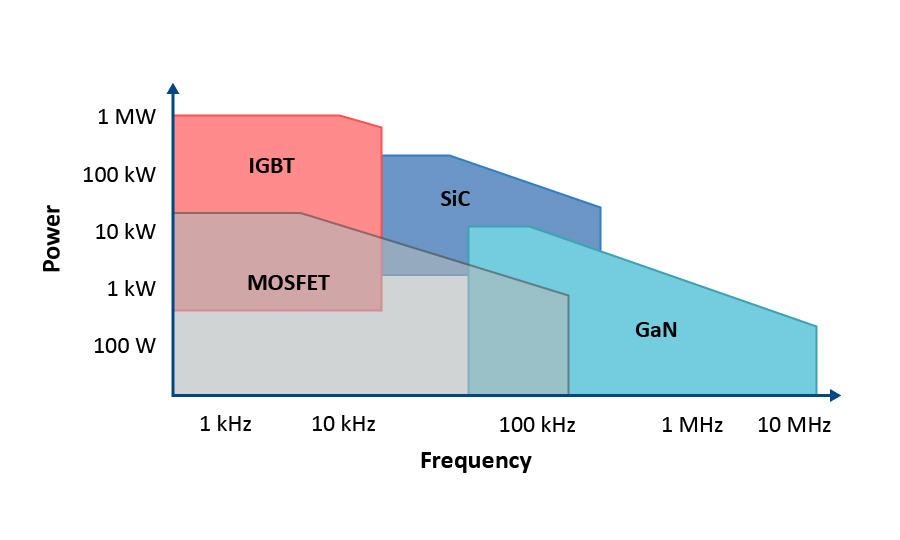
\includegraphics[width=0.6\textwidth]{Images/Implementation/tescnologies.jpg}
        \caption{Technologies selection based on power and switching frequency \cite{talat2024igbt}.}
        \label{fig:tech_transistor}
    \end{figure}


\section{Processing unit}
The processing unit runs the \ac{mppt} algorithm, generates the PWM signals and handles sensing, protection and communication. This section describes the microcontroller selection and its configuration.

    \subsection{MCU selection}

        A \acf{mcu} typically consists of three fundamental components: a central processing unit (CPU), memory, and peripheral modules. The CPU executes program instructions and performs arithmetic and logical operations. Memory is generally divided into non-volatile memory (Flash) for program storage and volatile memory (SRAM) for data and runtime variables. Peripheral modules provide interfaces to the external environment and may include analog-to-digital converters (ADCs), timers, pulse-width modulation (PWM) units, communication interfaces (such as UART, SPI, I²C and \acs{can}), and general-purpose input/output (GPIO) ports. Integrating these components enables standalone operation without extensive external circuitry~\cite{ibm_microcontroller_2025}.

        When selecting a \acs{mcu} for a specific application, the first factor to consider is to use an 8, 16, or 32 bit \acs{mcu}. For this application, a 16-bit \acs{mcu} would probably be sufficient, however to ensure future-proof and compatibility with other \ac{tsb} systems, the choice is for a 32-bit \ac{mcu}. Besides, nowadays, 32-bit \acp{mcu} are considered the industry standard since most embedded system \ac{red} effort is focused on 32-bit cores, and thus both architectures can achieve similar power consumption~\cite{embedded_upgrading_mcu_designs_2025}.
          There are two main architectures for 32-bit \acp{mcu}: AVR and ARM. Being the most widely used and most advanced architecture in the industry, ARM was chosen for this project~\cite{ampheo_fpga_vs_microcontroller_2025}. 

        STM32 is a family of \acp{mcu} that offers a wide range of solutions with different characteristics, making it suitable for various applications, including this project. \ac{tsb} uses this family of microcontrollers, so it will be the one used in this project to maintain the standard. 

        The \ac{mcu} requirements for this project are:
        \begin{itemize}[leftmargin=4em, itemsep=1pt, topsep=2pt]
            \item Fast clock frequency: 80~MHz or higher;
            \item Support 1x CAN peripheral, 1x I2C, 1x UART;
            \item Able to read 4 or more analog signals;
            \item 12bit ADC or more.
        \end{itemize}

        The final decision was the STM32L476. Although it is not the most suitable STM32 microcontroller for this application, it was selected due to its low cost and because it was already widely used within \ac{tsb}, reducing development time and associated risks.

        The STM32L476 is based on an ARM Cortex-M4 core with floating-point support and operates at frequencies up to 80~MHz. The device provides 1~MB of Flash memory and 128~kB of SRAM, which is more than sufficient for implementing the \ac{mppt} algorithm, data acquisition, communication protocols, and debugging features. Regarding peripherals, it includes three 12-bit ADCs with up to 16 external channels each, multiple general-purpose and advanced timers capable of high-resolution PWM generation, several communication interfaces (CAN, SPI, I\textsuperscript{2}C, UART, USB), and DMA controllers that allow peripheral operation with minimal CPU intervention.

        These features make the STM32L476 particularly attractive for power electronics applications that require simultaneous voltage and current measurements, fast PWM generation, and real-time control execution. Furthermore, the hardware floating-point unit simplifies the implementation of control algorithms and numerical calculations.

        If there were no limitations, a microcontroller with a higher clock frequency would have been selected, increasing both PWM duty-cycle resolution and available computational power. Additionally, a device with native 16-bit ADCs would improve measurement accuracy and reduce quantization effects. Nevertheless, the STM32L476 provides sufficient performance and peripheral resources to meet this application's requirements.

    \subsection{Configuration}
        Since the designed board is custom-made, there is no pre-configuration of the \ac{mcu} in use. In this particular case, the STM32 project needs to be configured in a STM32CubeMX, which is a tool that simplifies the configuration process. This tool is used to define the clock frequency, peripherals working frequency, pin mapping (GPIOs, ADCs, UART, CAN, etc.) and respective configuration, Interrupts, Timers, PWMs, etc. This tool generates a project based on C programming language with all drivers and configurations needed. These files serve as a base for firmware development and can be modified during the project.

        As it is not feasible to describe all the configurations used, the following section focuses on those most relevant to the project.

        The \ac{mcu} runs at 80~MHz with an external 16~MHz ceramic resonator. This frequency is enough for the computational time and a minimal PWM resolution. It can be flashed using JTAG and it uses an Independent Watchdog (IWDG) time interrupt. The IWDG is a safety feature that resets the \ac{mcu} in case of a crash or infinite loops. It works by resetting the timer periodically in a specific part of the code, if the timer is not reset during a specified time period, the interrupt is triggered and the \ac{mcu} resets automatically.

        As for timers, one timer was configured with 100~kHz for PWM and two pins were configured as complementary PWMs with a specific dead time. To prevent cross conduction (both transistors in conduction at the same time), the dead time was used as a safety feature too. The dead time is calculated using Formula~\ref{eq: dead time}, where the "value" must be in the range 0 to 255. 

        \begin{equation}
            Dead Time = Value / F_{CLK}
            \label{eq: dead time}
        \end{equation}
        
        For this project, several values were tested using an oscilloscope. The smallest value that ensures that both signals are never high at the same time is 2, however, 3 was used to add margin. The measured dead time was 32~ns, and the rise and fall times were 19~ns and 22~ns, respectively (Figure~\ref{fig:dead time}). 

        \begin{figure}[!ht]
            \centering
            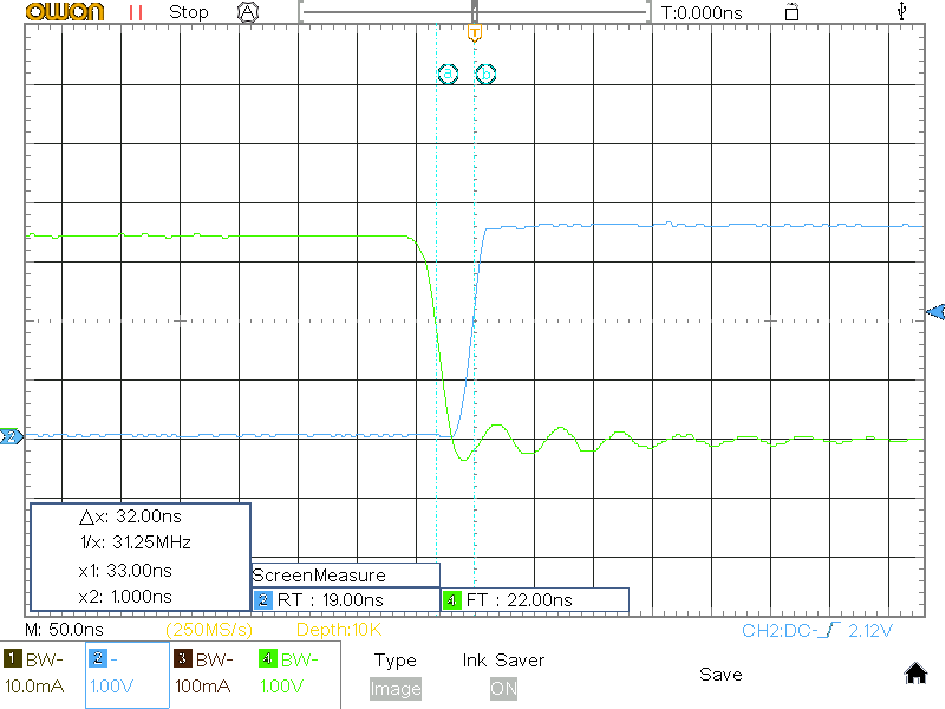
\includegraphics[width=0.6\textwidth]{Images/Implementation/dead3_zoom.pdf}
            \caption{Dead time measurement with oscilloscope (value=3).}
            \label{fig:dead time}
        \end{figure}

        In simulations, the dead time values of 2 and 3 were compared, and the difference in efficiency is only 0.01\%, and therefore the margin is justified. 

        With 100~kHz PWM and an 80~MHz internal clock, the duty cycle resolution is 0.125~\%.
        
        Another timer was configured to trigger every millisecond, and it is used to serve as task interrupts however, each task is called at different periods (always around milliseconds), which is implemented with a counters and comparators.

        The ADC can be configured in a variety of different ways, i chose to use the scan mode which reads multiple inputs in sequence. To read the measured values i am using the poling method however in theory if the DMA is used instead, the results could be better since it takes less time to read the ADC values and therefore a better average could be made. In practice i could not get reliable results and therefore the pooling method was adopted. The average is made with all data acquired between each \ac{mppt} algorithm call. 

\section{Sensors} 
The \ac{mppt} algorithm and the monitoring system rely on measurements of the electrical and environmental conditions of the system. This section describes the sensors used to measure the voltage and current at the converter's input and output, as well as the temperature and irradiance.

\subsection{Voltage and current sensing}
    Voltage sensing is generally straightforward and can be implemented using resistive voltage dividers followed by an ADC. Additionally, it is suggested to use an op-amp as a buffer to reduce the impact of the ADC input capacitor, while charging. This buffer reduces noise and improves the accuracy of the measurement while also allowing the use of higher sampling rates.
    
    Current sensing, however, is more critical and requires careful consideration of the available measurement techniques.

    The two main techniques are:
    \begin{itemize}[leftmargin=4em, itemsep=1pt, topsep=2pt]
        \item Hall effect current sensor;
        \item Shunt resistor sensing with operational amplifiers.
    \end{itemize}

    The Hall effect current sensor is a non-invasive method that uses the Hall effect to measure current. It provides galvanic isolation and can do bidirectional measurements. However, it is typically more expensive, has lower bandwidth, and may introduce additional noise due to its magnetic sensing nature.

    As for shunt resistor sensing, it is a simple and cost-effective method that uses a low value resistor to convert the current into a voltage drop. This voltage is then amplified using operational amplifiers to match the ADC input range. This method provides high accuracy, low cost, and fast-response time, but it requires careful design to minimize power loss, since it dissipates power proportional to the current.

    In the prototype, an \ac{ic} based on a shunt resistor sensing method was used, which has a built-in amplifier. The chosen sensor was the INA253A2IPWR, which has a PWM rejection block and a small form factor that will be extremely useful for this application. However, this \ac{ic} is more expensive than a simple shunt resistor and op-amp solution, but it is more accurate and has better noise rejection. In the future, it can be swapped for a lower cost solution if the performance is acceptable.

    Both sensors use the internal ADC from the STM32L476, which has a 12 bit ADC (with 3.0~V as the reference). The current sensor outputs an analog voltage that is equal to the current multiplied by 0.2~V/A. This means that the resolution of the measured current is 3.0/(4096 * 0.2) = 3.66~mA. As for the voltage sensor, it outputs an analog voltage that is equal to the voltage multiplied by 10/210. The resolution is 21 * 3.0/(4096) = 15.38~mV, which is more than enough for this application.

    Both circuits are represented in Appendix~\ref{chapter:Schematics}.

\subsection{Temperature and irradiance sensors}
    For security reasons, it is important to monitor the temperature of the \ac{pcb}. Also, monitoring the temperature and irradiance of the \ac{pv} panel is important for performance analysis and defect detection. These measurements can also be used to improve the \ac{mppt} algorithm, since the \ac{mpp} is dependent on temperature and irradiance.

    For temperature sensing, there is a wide range of options, from simple thermistors to more complex digital temperature sensors. For this application, it was used a simple thermistor because it is cheap and easy to implement. The thermistor is connected to a voltage divider and the voltage is read by the ADC. The thermistor used to measure ambient temperature and transistor temperature was the ERT-J1VS104FA, which has a resistance of $100~\mathrm{k}\Omega$ at $25~^\circ\mathrm{C}$ and a B value of 4330~K. The thermistor used to measure the \ac{pv} panel temperature is the 104JT-025, with a resistance of $100~\mathrm{k}\Omega$ at $25~^\circ\mathrm{C}$ and a B value of 4390~K. 
    The temperature can be calculated using the Steinhart-Hart equation \cite{arduinodiy2015ntc}.

    \begin{equation}
        \frac{1}{T} = A + B \cdot ln(R) + C \cdot ln(R)^3
    \end{equation}

    This equation uses 3 parameters (A, B and C) that are usually not provided in the datasheet but can be calculated using 3 measurements of temperature and resistance. However, the most common approach is to use a simplified version of the equation, which uses only 2 parameters (B and R0). The temperature can be calculated using the following equation:

    \begin{equation}
        \frac{1}{T} = \frac{1}{T_0} + \frac{1}{B} \cdot ln(\frac{R}{R_0})
    \end{equation}

    The thermistor that measures the transistor temperature is also used in analog protection. This protection uses a comparator to disable the transistors after a temperature threshold that can be modified by changing one resistor in the comparator circuit (Appendix~\ref{chapter:Schematics}). 

    As for the irradiance sensor, the board was designed to use a TSL2591, which is a digital light sensor with a wide dynamic range and high sensitivity. It can measure light intensity from 0.000118 lux to 88,000 lux, making it suitable for a wide range of lighting conditions. The sensor communicates with the \ac{mcu} via the I2C protocol, allowing for easy integration and data acquisition. However, this sensor is not ideal for outdoor use, since it can easily saturate and its spectrum is not ideal for solar irradiation measurement. The best application for this sensor is in laboratory, however, it was not needed, and therefore it was not used

    In the future, if the irradiance value needs to be used in the \ac{mppt} algorithm, a more precise irradiance sensor is needed. The most precise sensors use a \ac{pv} cells, which based on its temperature, short circuit current and open circuit voltage can provide a good estimation of the irradiance. The design of this circuit using the same cell model used in the \ac{pv} panel would accurately measure irradiance and have exactly the same spectral distribution as the \ac{pv} panel, which can be used for certain algorithms like \ac{lut}. This was not implemented in this project due to time constraints, but it is a good option for future work.


\section{Software}
    This section explains how the firmware inside the \ac{mcu} is structured and how it works. Also, the basic idea behind the communication protocols used and how they are applied to this project as well as the \ac{gui} developed for configuration and data analysis. 
    
    \subsection{Firmware overview}
        The firmware uses a flag-based scheduler with four tasks, shown in Figure~\ref{fig:Firmware flowchart}: ADC (1~ms), \ac{mppt} (20~ms), \acs{can} (100~ms) and serial (1~s). The periods are user configurable, originally the \ac{mppt} period was set to 10~ms (as it is in simulations) and increased to 20~ms to improve the measurement accuracy by increasing the number of samples taken. A 1~s watchdog timer resets the \ac{mcu} if a task crashes or enters infinite loops. 

        The fastest of these is the ADC task, which converts the analogue readings into current, voltage and temperature. If any value exceeds the configured limits, a fault is raised and the charging state machine is blocked for 5~s. After this delay the ADC task runs again and checks whether the faults have cleared. 

        \begin{figure}[!ht]
            \centering
            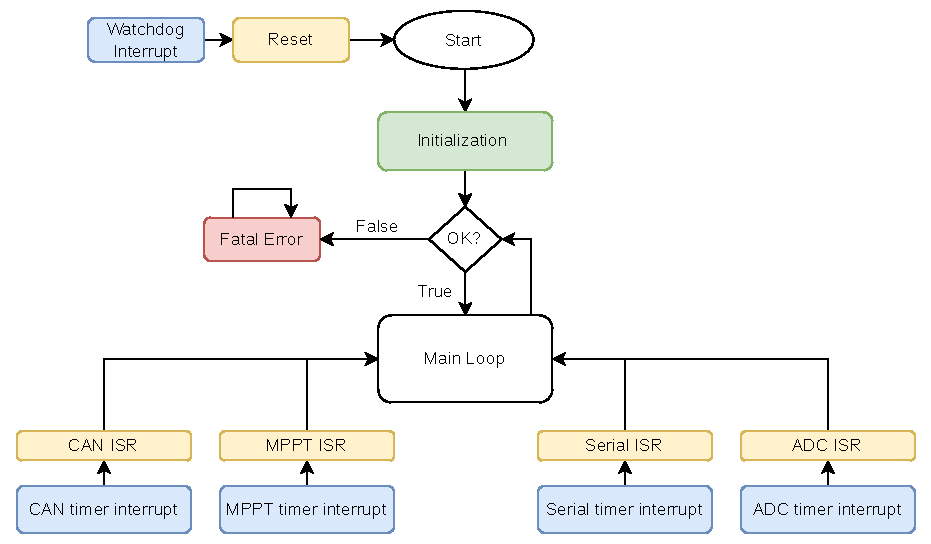
\includegraphics[width=0.6\textwidth]{Images/Implementation/Block diagram-Firmware_flowchart.drawio.pdf}
            \caption{Firmware flowchart.}
            \label{fig:Firmware flowchart}
        \end{figure}
        
        The \ac{mppt} task is responsible for computing an average of the last measurements and refreshing the state machine, which changes the operation mode depending on the measurements and outputs a PWM duty cycle value. In Figure~\ref{fig: charging state machine}, is represented the flow chart of the \ac{mppt} task state machine. 

        \begin{figure}[!ht]
            \centering
            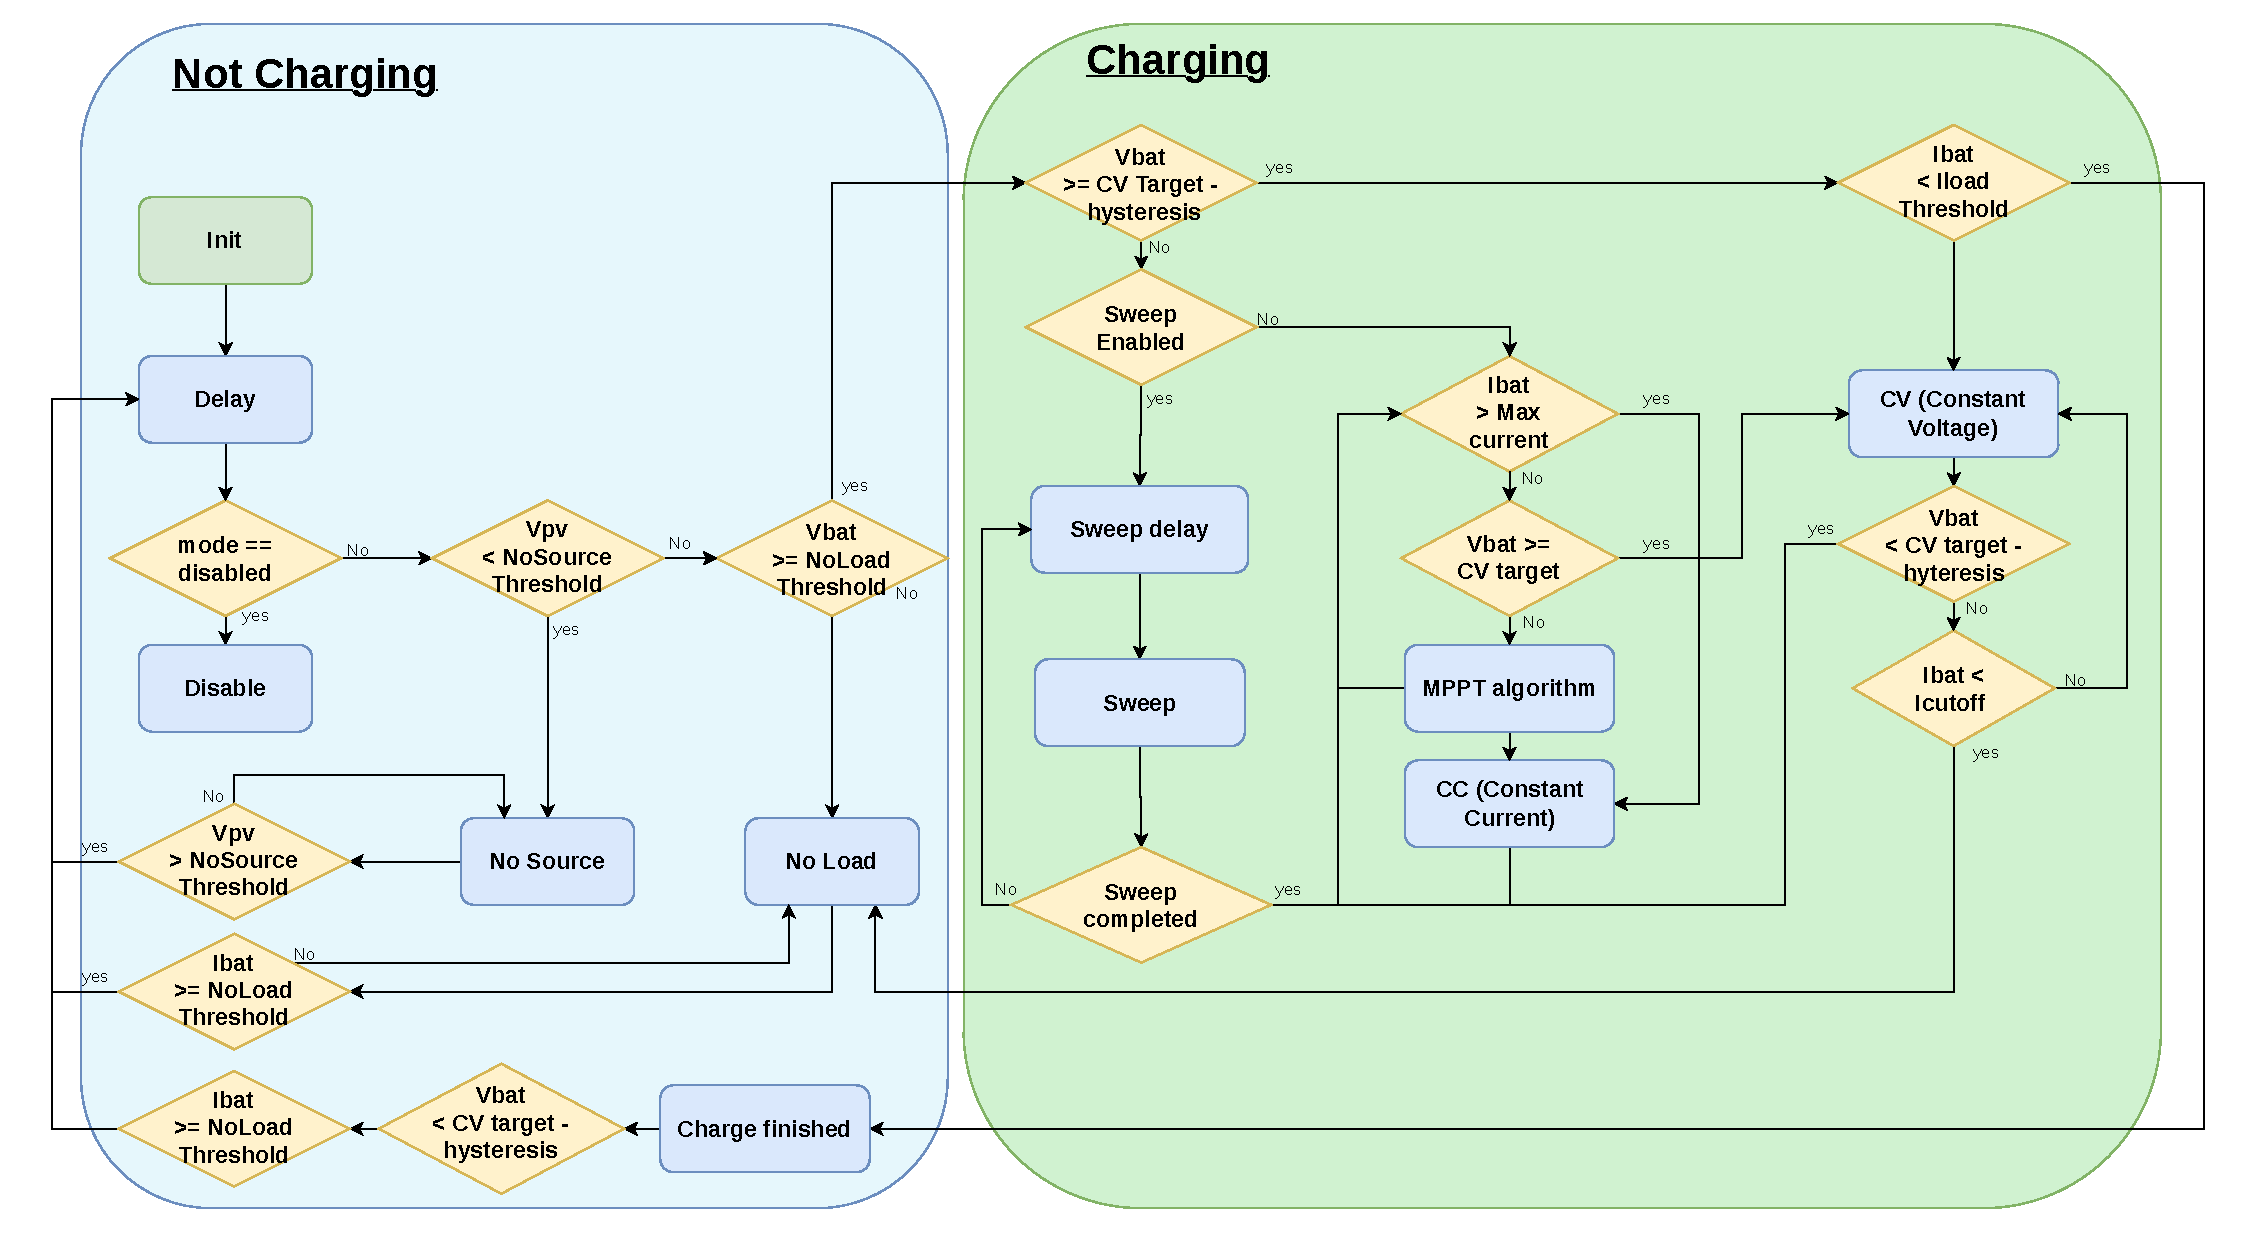
\includegraphics[width=0.9\textwidth]{Images/Implementation/MPPT_state_machine.drawio.pdf}
            \caption{Charging state machine.}
            \label{fig: charging state machine}
        \end{figure}

        The states are divided into charging and not charging. There are 5 "not charging" states:
        \begin{itemize}[leftmargin=4em, itemsep=1pt, topsep=2pt]
            \item \textbf{Delay}: waits 200 cycles (4~s) to skip the transients and then decides the next state. This state is important to let the output capacitors discharge when load is disconnected, therefore enabling the detection of the "No load" state;
            \item \textbf{Disable}: disables the \acs{dc}-\acs{dc};
            \item \textbf{No Source}: the solar panel is disconnected and therefore the \acs{dc}-\acs{dc} is disabled;
            \item \textbf{No load}: the battery is disconnected, and therefore the output voltage is set to the maximum battery voltage to prevent the need for a precharge circuit;
            \item \textbf{Charge finished}: similar to "No load", runs a proportional controller to follow the maximum battery voltage to prevent the need for a precharge.
        \end{itemize} 

        As for the charging states, there are also five:
        \begin{itemize}[leftmargin=4em, itemsep=1pt, topsep=2pt]
            \item \textbf{Sweep delay}: wait between sweep steps to ignore transients;
            \item \textbf{Sweep}: decrease the duty cycle until the end of the sweep. The sweep is used to find a true \ac{mpp} and ignore local maximums generated by partial shading;
            \item \textbf{MPPT algorithm}: runs the \ac{mppt} algorithm chosen;
            \item \textbf{CC}: if the current exceeds the battery limit, runs a proportional controller to follow the maximum current allowed;
            \item \textbf{CV}: runs a proportional controller to control the \acs{pv} side by following the battery voltage.
        \end{itemize}


    \subsection{Serial and CAN communication}
        One of the most important features of this circuit board is the communication with the rest of the boat. This will enable better decision making relating to the energy budget. Also, it will be easier to detect broken or malfunctioning solar panels or human errors such as bad or forgotten connections.

        The main communication protocol is \ac{can}. This is the \ac{tsb} standard protocol and is widely used in the automotive industry due to its high robustness. The protocol was developed by Bosch in 1986 to let microcontrollers and devices talk to each other without a central host computer. 
        
        From a hardware point of view, \ac{can} uses a bus instead of wire to wire communication. It also uses twisted wires (\ac{can} High and \ac{can} Low) to reduce electrical noise. From a software point of view, it uses an error checking system (CRC) ensuring reliability.

        For \ac{tsb} electrical system, it was developed a \ac{can} protocol on top of the standard \ac{can} communication. Each message is structured as shown in Figure~\ref{fig:can_protocol} following the \ac{can} 2.0A standard.
        
        \begin{figure}[!ht]
            \centering
            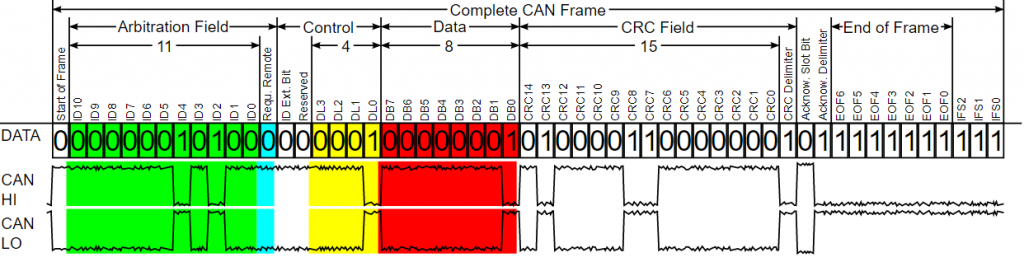
\includegraphics[width=0.85\textwidth]{Images/Implementation/CAN protocol.png}
            \caption{CAN protocol structure.}
            \label{fig:can_protocol}
        \end{figure}
        
        The 11 bits marked in green (Arbitration Field) can be used by each protocol differently. Usually, it is used to send priority bits, device ID and message ID. In the current vessel (\ac{sg01}), the priority bits were removed and used to increase the number of devices on the bus. With the current structure, represented in Table~\ref{tab:Arbitration Field}, the protocol supports up to 32 devices, each with 63 messages. 

        \begin{table}[!ht]
            \caption{\ac{tsb} CAN messages arbitration field.}
            \centering
            \begin{tabular}{|c|c|}
            \hline
            Message ID & Device ID \\
            \hline
            6 bits & 5 bits \\
            \hline
            \end{tabular}
            \label{tab:Arbitration Field}
        \end{table}

        In the Control field, the first bit indicates whether to use Extended IDs, and the next bit is reserved. The yellow field is called Data Length Code (DLC) and is where the length of the data is defined. The maximum length is 8 bytes. Then there is the Data field (represented in red). 

        The rest of the fields are treated by the \ac{can} library which is an adaptation of the open source library called \texttt{STM32\_CAN} by pazi88.

        For the \ac{mppt} it was defined an ID structure, where the device ID is maintained intact, and Message ID is divided in two. The 3 most significant bits represent the \ac{mppt} number from 0 to 7, and the remaining bits identify the messages. This structure provides enough message IDs for each \ac{mppt} as well as not occupying a lot of Device IDs. Table~\ref{tab:mppt_message_ids} shows an example of the corresponding IDs when the Device ID is 0x0D (default ID).

        \begin{table}[!ht]
            \caption{CAN IDs for each MPPT number and message.}
            \centering
            \begin{tabular}{|c|c|c|c|c|}
                \hline
                \textbf{MPPT Number} & \textbf{MSG:MPPT\_bat} & \textbf{MSG:MPPT\_pv} & \textbf{MSG:MPPT\_aux1} & \textbf{MSG:MPPT\_aux2} \\
                \hline
                \textbf{0} & \texttt{0x00D} & \texttt{0x02D} & \texttt{0x04D} & \texttt{0x06D} \\
                \hline
                \textbf{1} & \texttt{0x10D} & \texttt{0x12D} & \texttt{0x14D} & \texttt{0x16D} \\
                \hline
                \textbf{2} & \texttt{0x20D} & \texttt{0x22D} & \texttt{0x24D} & \texttt{0x26D} \\
                \hline
                \textbf{3} & \texttt{0x30D} & \texttt{0x32D} & \texttt{0x34D} & \texttt{0x36D} \\
                \hline
                \textbf{4} & \texttt{0x40D} & \texttt{0x42D} & \texttt{0x44D} & \texttt{0x46D} \\
                \hline
                \textbf{5} & \texttt{0x50D} & \texttt{0x52D} & \texttt{0x54D} & \texttt{0x56D} \\
                \hline
                \textbf{6} & \texttt{0x60D} & \texttt{0x62D} & \texttt{0x64D} & \texttt{0x66D} \\
                \hline
                \textbf{7} & \texttt{0x70D} & \texttt{0x72D} & \texttt{0x74D} & \texttt{0x76D} \\
                \hline
            \end{tabular}
            \label{tab:mppt_message_ids}
        \end{table}

        The Device ID can be configured/changed via \ac{gui} however, the logic is maintained.

        The CAN protocol is excellent for communication between boards, however, it is not the most practical protocol for configuration because the \ac{can} IDs can change between vessels and imply the use of an external hardware to communicate between the board and a computer.

        In contrast, serial communication is done by just connecting a cable to the board, and since the protocol is only used for configuration and data analysis, it can be the same forever, and if it needs to be changed, it does not depend on any vessel. 

        There is no default protocol to send data over serial, however, during the \ac{bms} thesis a serial protocol was created by the team and will serve has based for this project. Unfortunately, the firmware library is not compatible with STMs, so it was created from scratch.

        The protocol uses the structure defined in Table~\ref{tab:serial_message_format}. It begins with the Start Byte, which is defined as 0xAC, followed by the device ID, which defines the source of the message, and the message ID, defining what message the device is sending, the data length, the data, the checksum byte, and the end byte (0xAD) marking the end of the message.

        \begin{table}[!h]
            \centering
            \caption{\ac{tsb} Serial messages format.}
            \label{tab:serial_message_format}
            \begin{tabular}{|c|c|c|c|c|c|c|}
                \hline
                \textbf{Start} & \textbf{Device ID} & \textbf{MSG ID} & \textbf{LEN} & \textbf{Data} & \textbf{Checksum} & \textbf{END} \\ \hline
                1 Byte & 1 Byte & 1 Byte & 1 Byte & 8 Bytes & 1 Byte & 1 Byte \\ \hline
            \end{tabular}
        \end{table}
        
        Similar to the CAN protocol, for each message, a Message ID was defined respecting the same logic. This ID, alongside with the Device ID and length, is initialized at the beginning of the code, the rest of the variables are handled by the library, except the data field which is changed before sending any message.
        
        The Data of each message is structured in the same way as in \ac{can} protocol however it was added 4 messages for configuration. These messages enable the change of current limits, voltage limits, \ac{mppt} parameters, \ac{can} settings and CC-CV targets.
        

    \subsection{EEPROM emulation}
        To save the configuration received from the serial protocol, a library was used that emulates an EEPROM, which is a type of non-volatile memory that retains its contents after power down. EEPROMs have been used for many years in a wide range of devices to store settings, calibration data, and backups. In this project, no external EEPROM was added to the board, and the \ac{mcu} does not include one internally. However, the library can use internal flash memory, which is normally reserved for the flashed code, to store data, thereby emulating EEPROM behavior.

        The main disadvantages of this approach are limited storage capacity and reduced write endurance compared with a dedicated EEPROM. The STM32 internal flash can typically withstand on the order of 10,000 erase cycles per page, whereas external EEPROM devices often support roughly one order of magnitude more. Even so, this is not a practical limitation in this application. Configuration data is stored as a small set of 16-bit variables, and each save operation appends new records to flash rather than overwriting the previous value in place. Each page can hold 252 variables. For this project, a full board configuration requires 13 write operations, therefore, one flash page can hold many configuration updates before it becomes full and must be erased. Furthermore, the emulation is configured to use ten flash pages, with wear leveling implemented through page transfer and cleanup. When a page is full, the latest values are copied to another page and the old page is eventually erased. This distributes erase cycles across multiple pages and extends the effective lifetime of the memory.

        In conclusion, neither storage capacity nor endurance is expected to be a problem for this project. Under the current configuration, a complete configuration upload would need to be performed hundreds of thousands of times before the theoretical endurance limit of a flash page is reached, which is far beyond the expected use case of occasional configuration updates over serial.

        Since the emulated EEPROM shares the same physical flash as the firmware, care must be taken to ensure that program code is never placed in the reserved EEPROM region. This was achieved by modifying the linker script, which defines the memory map used during the build process. The length of the program flash region was reduced so that firmware is linked only below the first address saved for EEPROM emulation.

        Two additional mechanisms were implemented to protect the emulated EEPROM from accidental corruption. The first is a magic word that is written to the first address of each page. This is a fixed 16-bit signature that indicates that the page was written by valid firmware rather than left as uninitialized or partially erased flash. The second is a validation process. Each variable is only considered valid if it is within the specified range.


    \section{Graphical User Interface}
        In parallel with the design and test of the \ac{mppt} board, a \ac{gui} was designed to make the project more accessible and easy to use. The application was built from scratch, however it was inspired in the application built during \ac{bms} thesis. It was built using QT framework, which is a powerful, cross platform software toolkit used to build high performance applications and \acp{gui} that run on multiple operating systems like Windows, macOS and Linux. 

        This \ac{gui} communicates with the board with Serial or \ac{can} communication. To use \ac{can} communication, the computer should be connected to the bus with a tool called PEAK-CAN.
        
        After connecting the computer to the board, the application identifies the connected board and shows it to the user on the Dashboard page (Figure~\ref{fig:Dashboard}).On the main page, the user selects which board he is working on. The application is prepared for several \acp{pcb}, however, only the \ac{bms} and \ac{mppt} are correctly working. The rest are placeholders for future improvements.

        When the \ac{mppt} page is selected (Figure~\ref{fig:MPPT monitor GUI}), a new tab opens showing the most important variables, such as voltage, current, power, temperature, efficiency, irradiance, and duty cycle. Additionally, two visual representations are shown. On the left, a P-V graph shows theoretical curves for different irradiance values, with a blue dot at the current operating point that updates with the received data.

        On the right, the CC-CV curve is represented, where the received battery side data is shown over time.

        \begin{figure}[!ht]
            \centering
            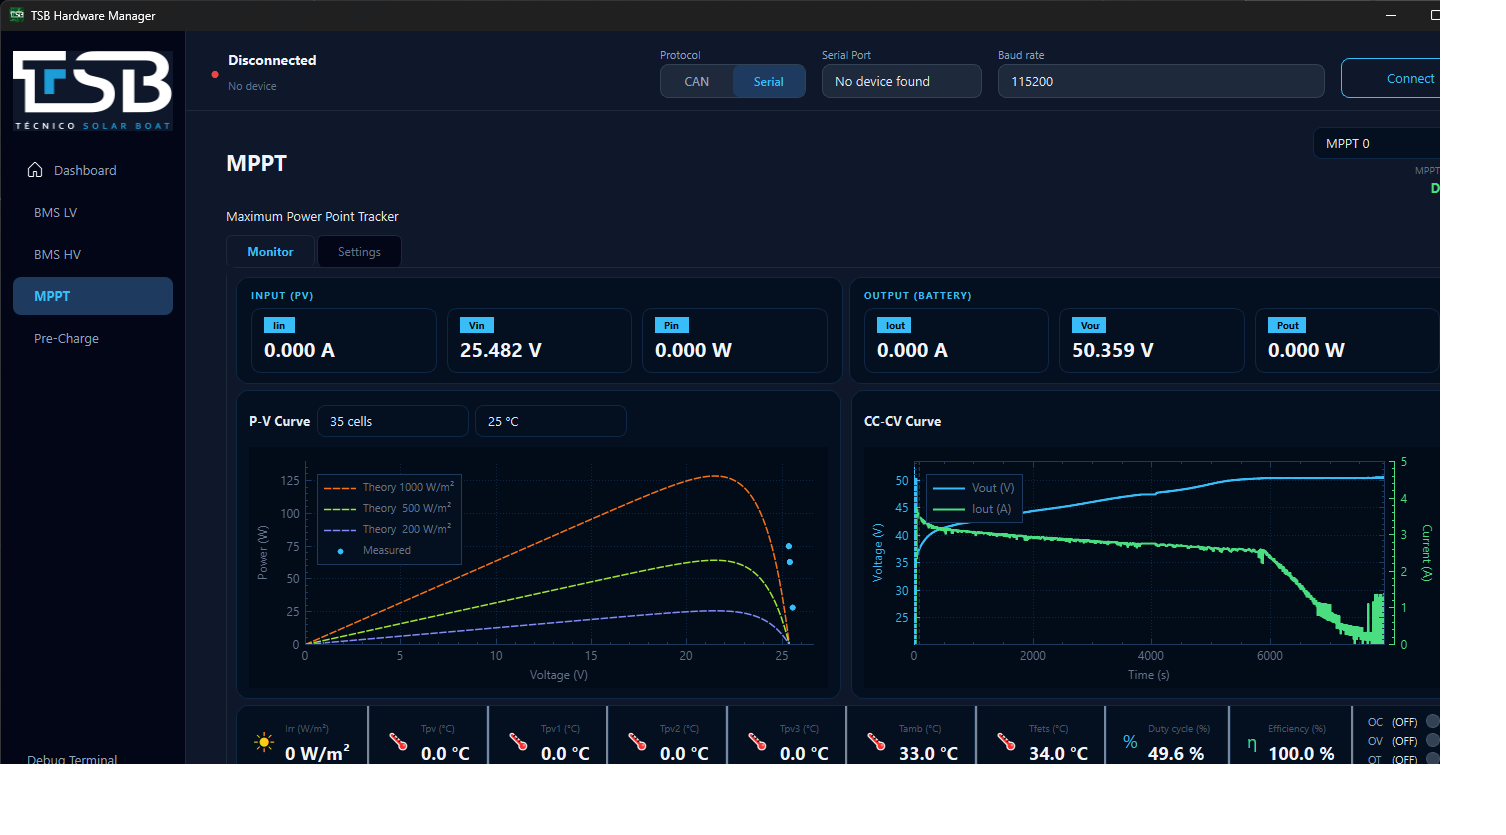
\includegraphics[width=0.90\textwidth]{Images/Implementation/GUI_MPPT_main.png}
            \caption{MPPT monitor tab.}
            \label{fig:MPPT monitor GUI}
        \end{figure}

        On top of the page, the user can switch to the configuration tab (Figure~\ref{fig:MPPT config tab}). In this tab, the user can read the configuration currently installed on the board, reset this configuration, or upload a new one.

        The last page is the debug page (Figure~\ref{fig:Debug page}), where the user can visualize both Serial protocol messages and serial prints at the same time.

 